\section{Response Time Model Creation}\label{model_creation}
To create RTF models either at install time or online we use a least squares approach described below.  For the install time approach we use a genetic algorithm, Audze-Eglasis Design of Experiments\cite{bates-aes03}, to select the resource vectors to use for training.  These vectors and their response times are fed into the least squares algorithm. In the online approach the information comes from the application's response time history.

\subsubsection*{Model Creation using Least Squares}
After enough measurements, discovery of the model parameters $w$ that define the function $\tau$
can be based on a solution to the over-determined linear system $t=Dw$,
where $t$ is a column vector of actual response times measured for the application
and $D$ is a matrix whose ith row $D_{i,*}$ contains the corresponding resource vector.
Estimating $w$ is relatively straightforward: a least-squares solution accomplished via
\emph{QR factorization}\cite{GoVL} of $D$ will determine the $w$ that minimizes the \emph residual error of
$\|Dw - t\|^2_2 =  \|\varepsilon\|^2_2$.
The solution proceeds as follows:
\begin{eqnarray*}
t     &=& Dw  - \varepsilon    \\
      &=& QRw - \varepsilon    \\
Q^Tt  &=& Rw  - Q^T\varepsilon
\end{eqnarray*}

The individual elementary orthogonal transformations, \emph{e.g.,} Givens rotations,
that triangularize $R$ by progressively zeroing out $D$'s sub-diagonal elements are simultaneously applied to $t$.
The elements of the resulting vector $Q^Tt$ that correspond to zero rows in $R$ comprise $-Q^T\varepsilon$.
Since $Rw$ exactly equals the upper part of $Q^Tt$, the upper part of $Q^T\varepsilon$ is zero. The residual error for the $t_i$
can be found by premultiplying $Q^T\varepsilon$ by $Q$.

%This formulation assumes a model norm $p = 1$. If a different model norm $p$ is desired, such as $p = 2$, we could first square %each measurement in $t$
%and each reciprocal bandwidth term in $D$ and then follow the foregoing procedure.
%The elements of the result $w$ will be squares as well, and the 2-norm of the difference in the squared quantities will be %minimized.  This is not the same as minimizing the 4-norm; what is being minimized is $1/2\|\mbox{diag}(Dww^TD^T - tt^T)\|^2_2$.

\subsection*{On-line Response Time Modeling}
As resource allocation continues, more measurements will become available to augment $t$ and $D$.
Moreover, older data may poorly represent the current behavior of the application.
\pacora uses an incremental approach described below to replace old data and efficiently update RTFs.

\subsubsection*{Incremental Least Squares}
What is needed is a factorization $\tilde{Q}\tilde{R}$ of a new matrix $\tilde{D}$
derived from $D$ by dropping a row, perhaps from the bottom,
and adding a row, perhaps at the top.
Corresponding elements of $t$ are dropped and added to form $\tilde{t}$.

The matrices $\tilde{Q}$ and $\tilde{R}$ can be generated by applying Givens rotations
in the way described in Section 12 of \cite{GoVL} to \emph{downdate} or \emph{update} the factorization
much more cheaply than recomputing it \emph{ab initio}.
The method requires retention and maintenance of $Q^T$ but not of $D$.
Every update in \pacora is preceded by a downdate that makes room for it.
Downdated rows are \emph{not} always the oldest (bottom) ones, but
an update always adds a new top row.
For several reasons, the number of rows $m$ in $R$
will be at least twice the number of columns $n$.
Rows selected for downdating will always be in the lower $m - n$ rows of $R$,
guaranteeing that the most recent $n$ updates are always part of the model.

%\subsubsection*{Non-Negativity}
%\begin{figure*}[!t]
%	\begin{center}	
%%		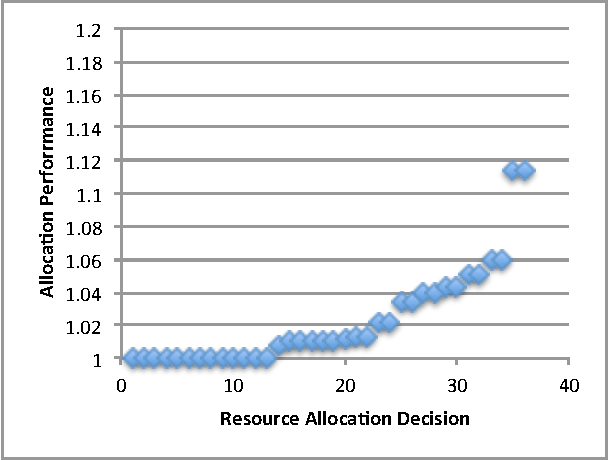
\includegraphics[width=.45\textwidth]{cluster_decision_points.pdf}
%		\caption{Performance of \pacora's NNLS algorithm}
%		\label{model_build_perf}
%	\end{center}
%\end{figure*}

To guarantee convexity of the RTF, the solution $w$ to $t \approx QRw$ must have no negative components.
Intuitively, when a resource is associated with more than a single $w_j$
or when the measured response time increases with allocation then negative $w_j$ may occur.

A requirement for non-negative solutions to least-squares linear algebra problems is common,
so much so that it has a name: \emph{Non Negative Least Squares}, or NNLS.
There are several well-known techniques\cite{ChPl},
but since \pacora's online model maintenance calls for
incremental downdates and updates to rows of $Q^T$, $Q^Tt$ and $R$,
the NNLS problem is handled with a scheme
based on the \emph{active-set} method\cite{LaHa} that
also downdates and updates the \emph{columns} of $R$ incrementally,
roughly in the spirit of Algorithm~3 in~\cite{LuDu}.
However, \pacora's algorithm cannot ignore downdated columns of $R$
because subsequent \emph{row} updates and downdates must have due effect
on these columns to allow their later reintroduction via column updates as necessary.
This problem is solved by leaving the downdated columns in place,
skipping over them in maintaining and using the QR factorization.

The memory used in maintaining a model with $n$ weights is modest, $24n^2 + 21n + \textrm{O}(1)$ bytes.
For $n = 8$ this is under 2 KB, fitting nicely in L1 cache.
Our NNLS implementation runs in around \fix{x $\micro$s}.
%Figure~\ref{model_build_perf} shows the performance of \pacora's NNLS algorithm.

\subsubsection*{Model Rank Preservation}
If care is not taken in downdating $R$, its rows may become so linearly dependent,
perhaps from repetitive resource allocations,
that determining a unique $w$ is impossible.
The rank of $R$ depends on both the resource optimization trajectory and the
choices made in the row downdate-update algorithm.
\pacora exploits the latter idea and simply avoids downdating any row that will make $R$ rank-deficient.

\subsubsection*{Outliers and Phase Changes}

%\begin{figure*}[!t]
%	\begin{center}	
%%		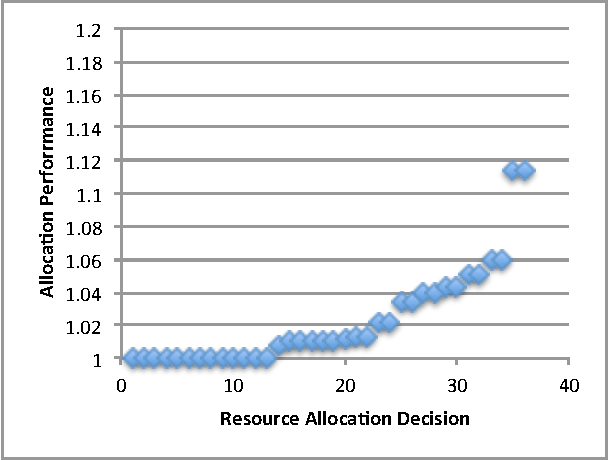
\includegraphics[width=.45\textwidth]{cluster_decision_points.pdf}
%		\caption{\pacora's online model creation algorithm adapting to a video application changing phases}
%		\label{phase_change}
%	\end{center}
%\end{figure*}

Some response time measurements may be ``noisy'' or even erroneous.
A weakness of least-squares modeling is the high importance it gives to outlying values.
On the other hand, when an application changes phase it is important to adapt quickly,
and what looks like an outlier when it first appears may be a harbinger of change.
What is needed is a way to discard either old or outlying data
with a judicious balance between age and anomaly.

The downdating algorithm accomplishes this by weighting the errors in $\varepsilon = Q(Q^Tt - Rw)$
between the predicted response times $\tau$ and the measured ones $t$ by a factor
that increases exponentially with the age $g(i)$ of the error $\varepsilon_i$.
Age can be modeled coarsely by the number of time quanta of some size since the measurement;
\pacora simply lets $g(i) = i$.
The weighting factor for the $i$th row is then $\eta^{g(i)}$ where $\eta$ is a constant somewhat greater than 1.
The candidate row to downdate is the row with the largest weighted error, \emph{i.e.,}
$dd = \arg\max_i |\varepsilon_i| \cdot \eta^{g(i)}$ and that does not reduce the rank of $R$.
%Figure~\ref{phase_change} shows \pacora's model creation algorithm adapting to a video application changing phases.


\subsubsection*{Power Response Modeling}
Recall that we manage power and battery energy with an artificial application named Application 0 which receives all resources not allocated to other applications. Application 0's "response time" function is similar to the other applications' response time functions.  The function inputs are resource allocations just as with the other applications.  However, the function output is system power rather than response time.   To create the RTF, system power can be measured directly from on-chip energy counters in systems where they are available or from a power meter.  These models can be built in advance, during a training phase or online while the system runs, just as with the application RTFs.  Alternatively, the model could be part of the operating system's platform-specific information.

Although system power may not be perfectly convex in reality, forcing it to be convex is reasonable because idling a resource should not increase power.  As a result, Application 0 still fills its purpose of keeping applications from using additional resources that have poor performance/power ratios.

